\documentclass[xcolor={svgnames}]{beamer}
\usetheme{CambridgeUS}
\usecolortheme{seagull}

\usepackage{amsfonts,amsmath,amsthm,amssymb}
\usepackage{graphicx}
\usepackage{array}
\usepackage{pgfpages}
\usepackage[square,authoryear]{natbib}
\usepackage{multicol}

\newtheorem{proposition}[theorem]{Proposition}%[section]
\newtheorem{conjecture}{Conjecture}%[section]

%\pgfpagesuselayout{2 on 1}[a4paper,border shrink=5mm]

%\newcommand{\alg}{\mathcal{A}}
\newcommand{\alg}{\mathcal{M}}
\newcommand{\eps}{\varepsilon}
\newcommand{\E}{\mathbb{E}}
\renewcommand{\vec}[1]{#1}

\DeclareMathOperator{\vollb}{volLB}
\DeclareMathOperator{\detlb}{detLB}
\DeclareMathOperator{\disc}{disc}
\DeclareMathOperator{\hd}{hd}
\DeclareMathOperator{\vb}{vb}
\DeclareMathOperator{\vol}{vol}
\DeclareMathOperator{\cov}{cov}
\DeclareMathOperator{\conv}{conv}
\DeclareMathOperator{\lspan}{span}


\DeclareMathOperator{\rank}{rank}

\DeclareMathOperator{\row}{row}
\DeclareMathOperator{\col}{col}


\DeclareMathOperator{\diag}{diag}


\newcommand{\R}{\mathbb{R}}
\newcommand{\BB}{\mathcal{B}}
\renewcommand{\SS}{\mathcal{S}}
\newcommand{\range}{\mathcal{R}}
\DeclareMathOperator{\tr}{tr}
\newcommand{\junk}[1]{}
\newcommand{\symdif}{\oplus}
\newcommand{\mycite}[1]{\textcolor{blue}{\citep*{#1}}}
\newcommand{\maps}{\colon}
\newcommand{\eqdef}{:=}

\definecolor{magenta}{HTML}{A52A2A}
\definecolor{seagreen}{HTML}{006400}

\newcolumntype{+}{>{\global\let\currentrowstyle\relax}}
\newcolumntype{=}{>{\currentrowstyle}}
\newcommand{\rowstyle}[1]{\gdef\currentrowstyle{#1}
  #1\ignorespaces
}


\title[Balancing Vectors]{Balancing Vectors in Any Norm}

\author[Sasho Nikolov]{\emph{Aleksandar (Sasho) Nikolov}}
\institute[U of T]{University of Toronto} 
\date{}

\begin{document}

\frame{\titlepage 
  \begin{center}Joint work with\smallskip\\
    Daniel Dadush (CWI), Kunal Talwar (Google), \\and Nicole
    Tomczak-Jaegermann (U Alberta)\bigskip\\
  \end{center}}

% \AtBeginSection[]
% {
%   \begin{frame}<beamer>
%     \frametitle{Outline}
%     \tableofcontents[currentsection]
%   \end{frame}
% }

\section{Introduction}

\frame{

  \frametitle{Discrepancy of Set Systems}
  \only<1>{\vspace{-1.8em}}
  Given: universe $\mathcal{X}$ of $N$ elements, and $n$ subsets $\SS=
  \{S_1, \ldots, S_n\}$ of $\cal X$. 

  Color each universe element \textcolor{red}{red} or
  \textcolor{blue}{blue}, so that \emph{each} set is as balanced as possible.

  \begin{center}
    \only<1>{
      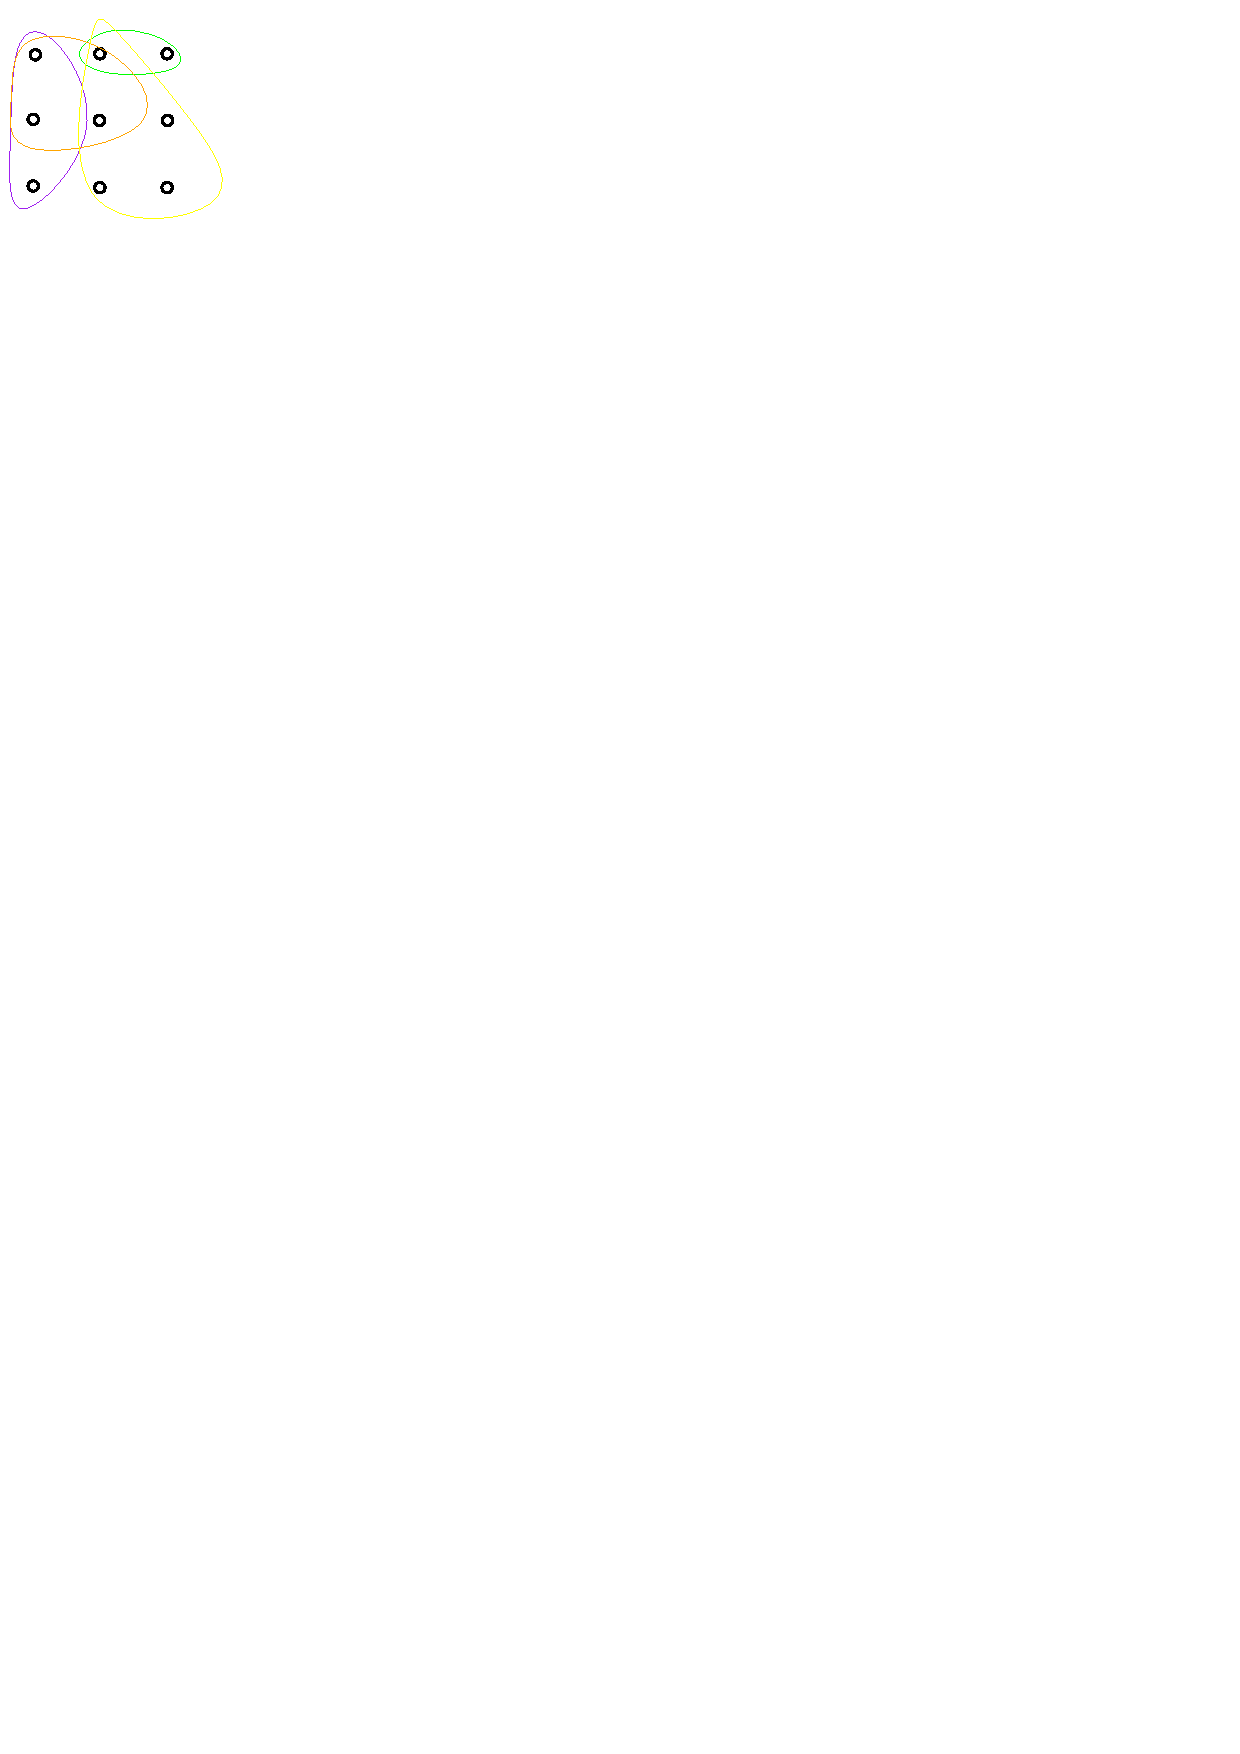
\includegraphics{setsystem}}
    \only<2>{
      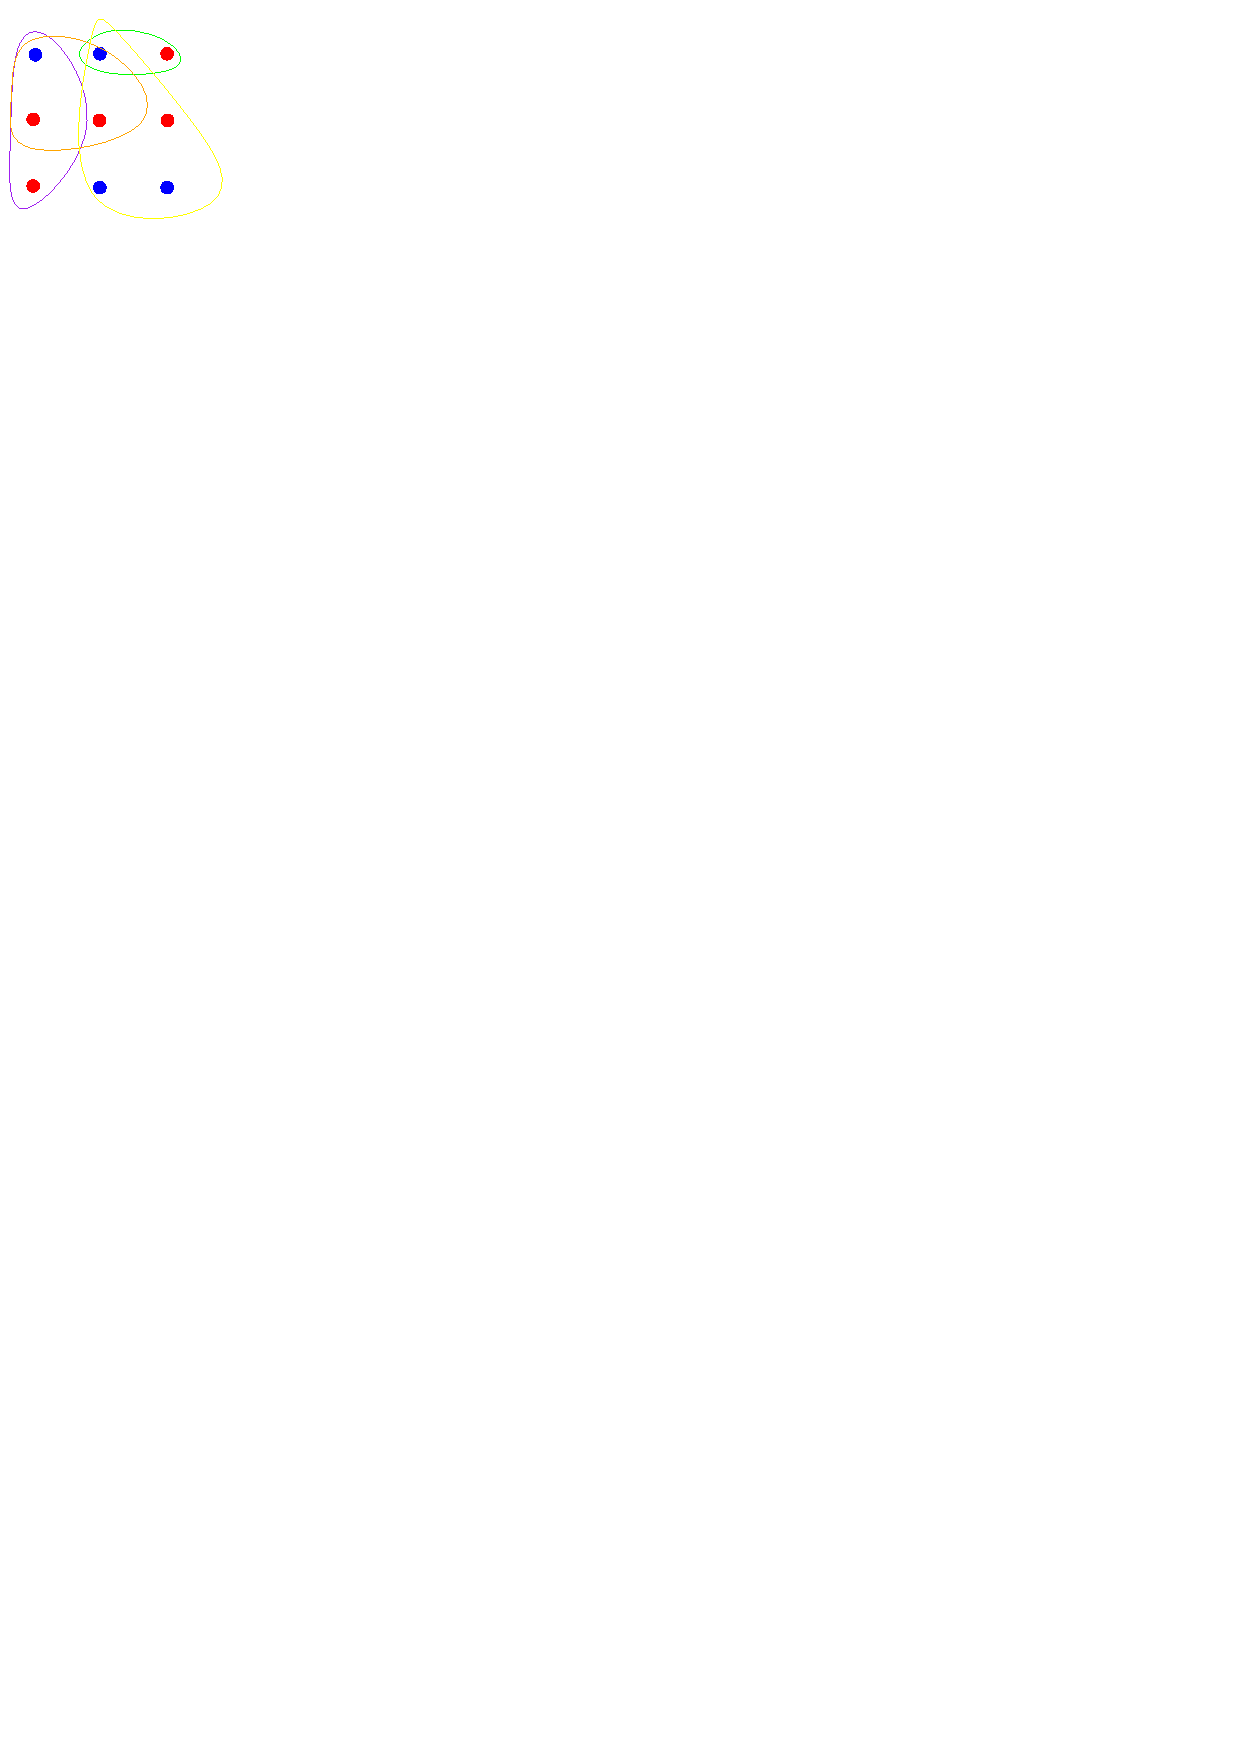
\includegraphics{setsystemcolored}    }
  \end{center}

  \only<2>{
    Discrepancy of a coloring: maximum imbalance (above: 1). 

    Dicrepancy of $\SS$: discrepancy of the best coloring. 
  }



}


\frame{

  \frametitle{Matrix Representation}

  \only<1>{
    \vspace{1.5em}
      \begin{center}
        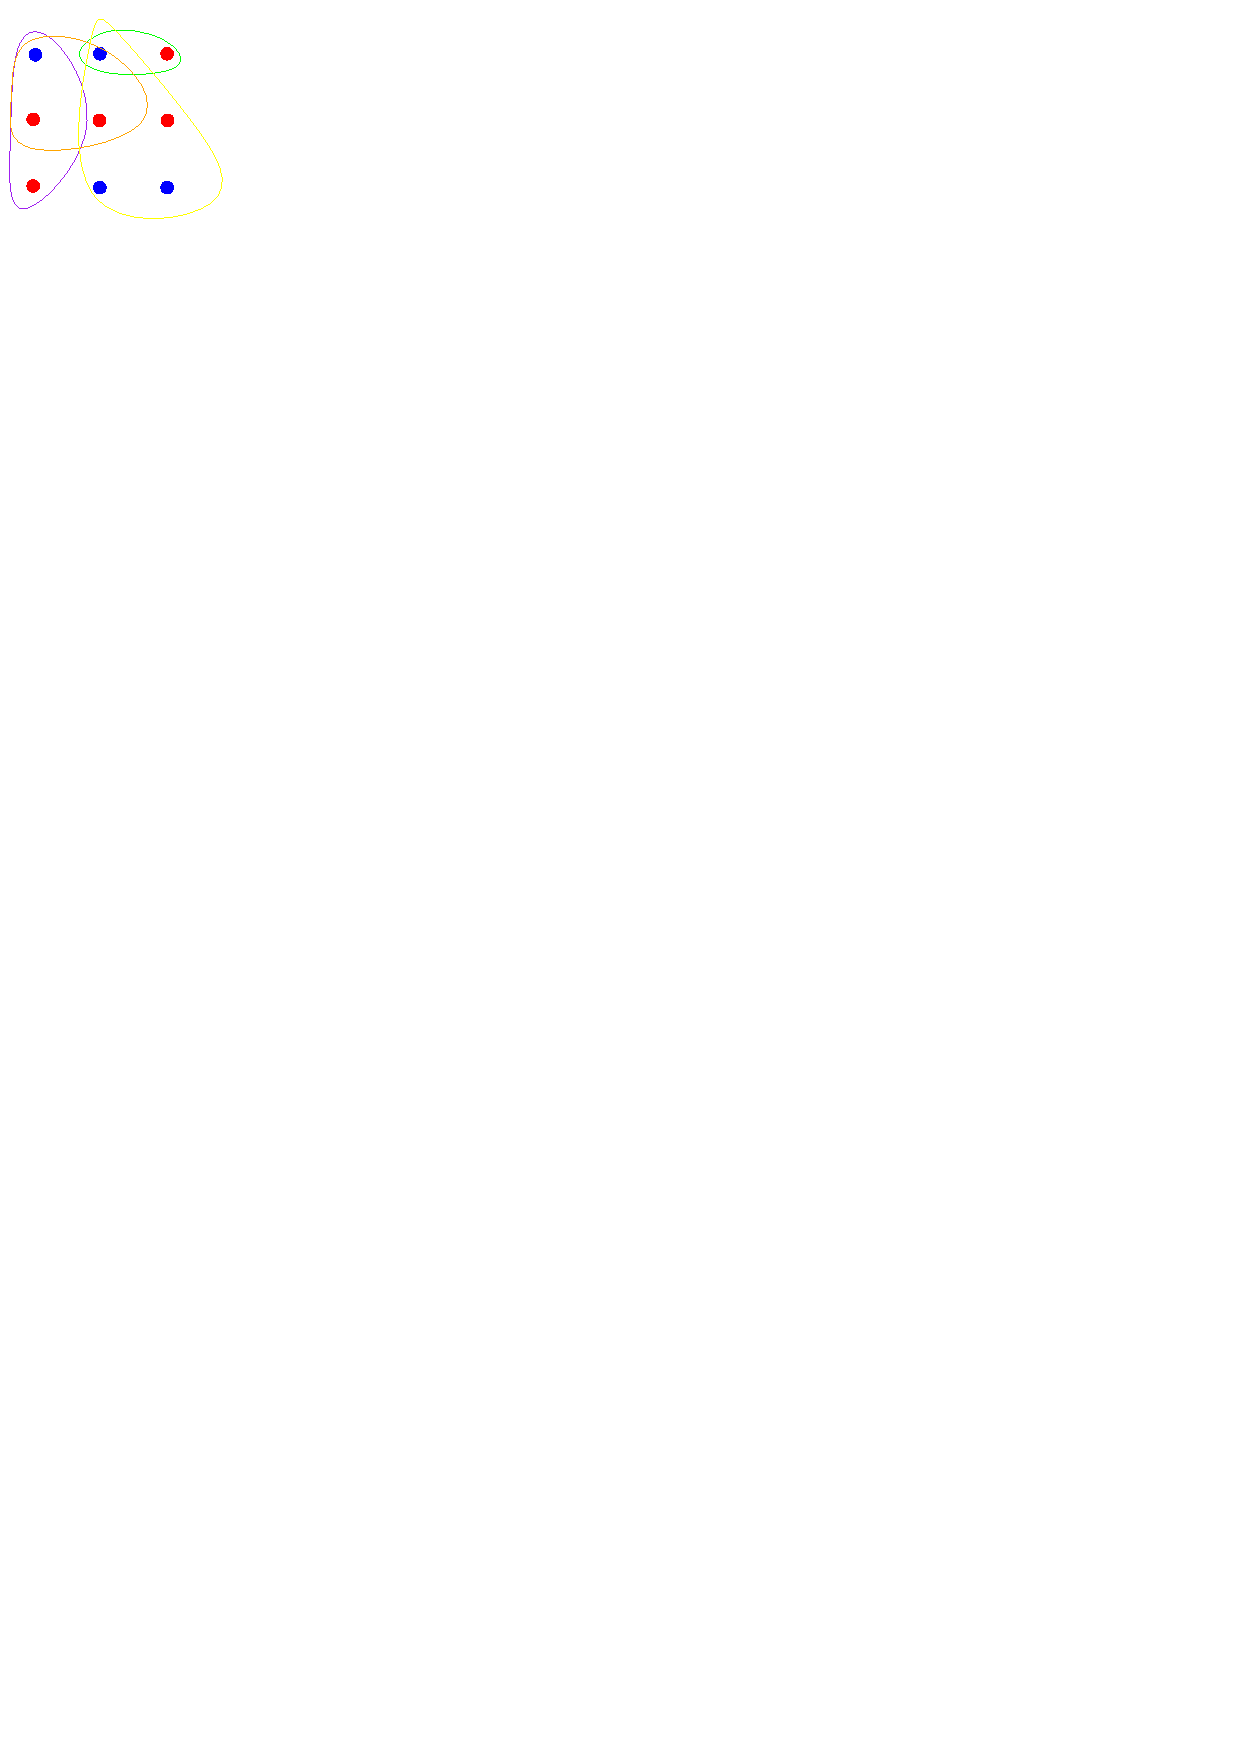
\includegraphics{setsystemcolored}    
      \end{center}
  }
  \only<2>{
    \vspace{1.5em}
      \begin{center}
        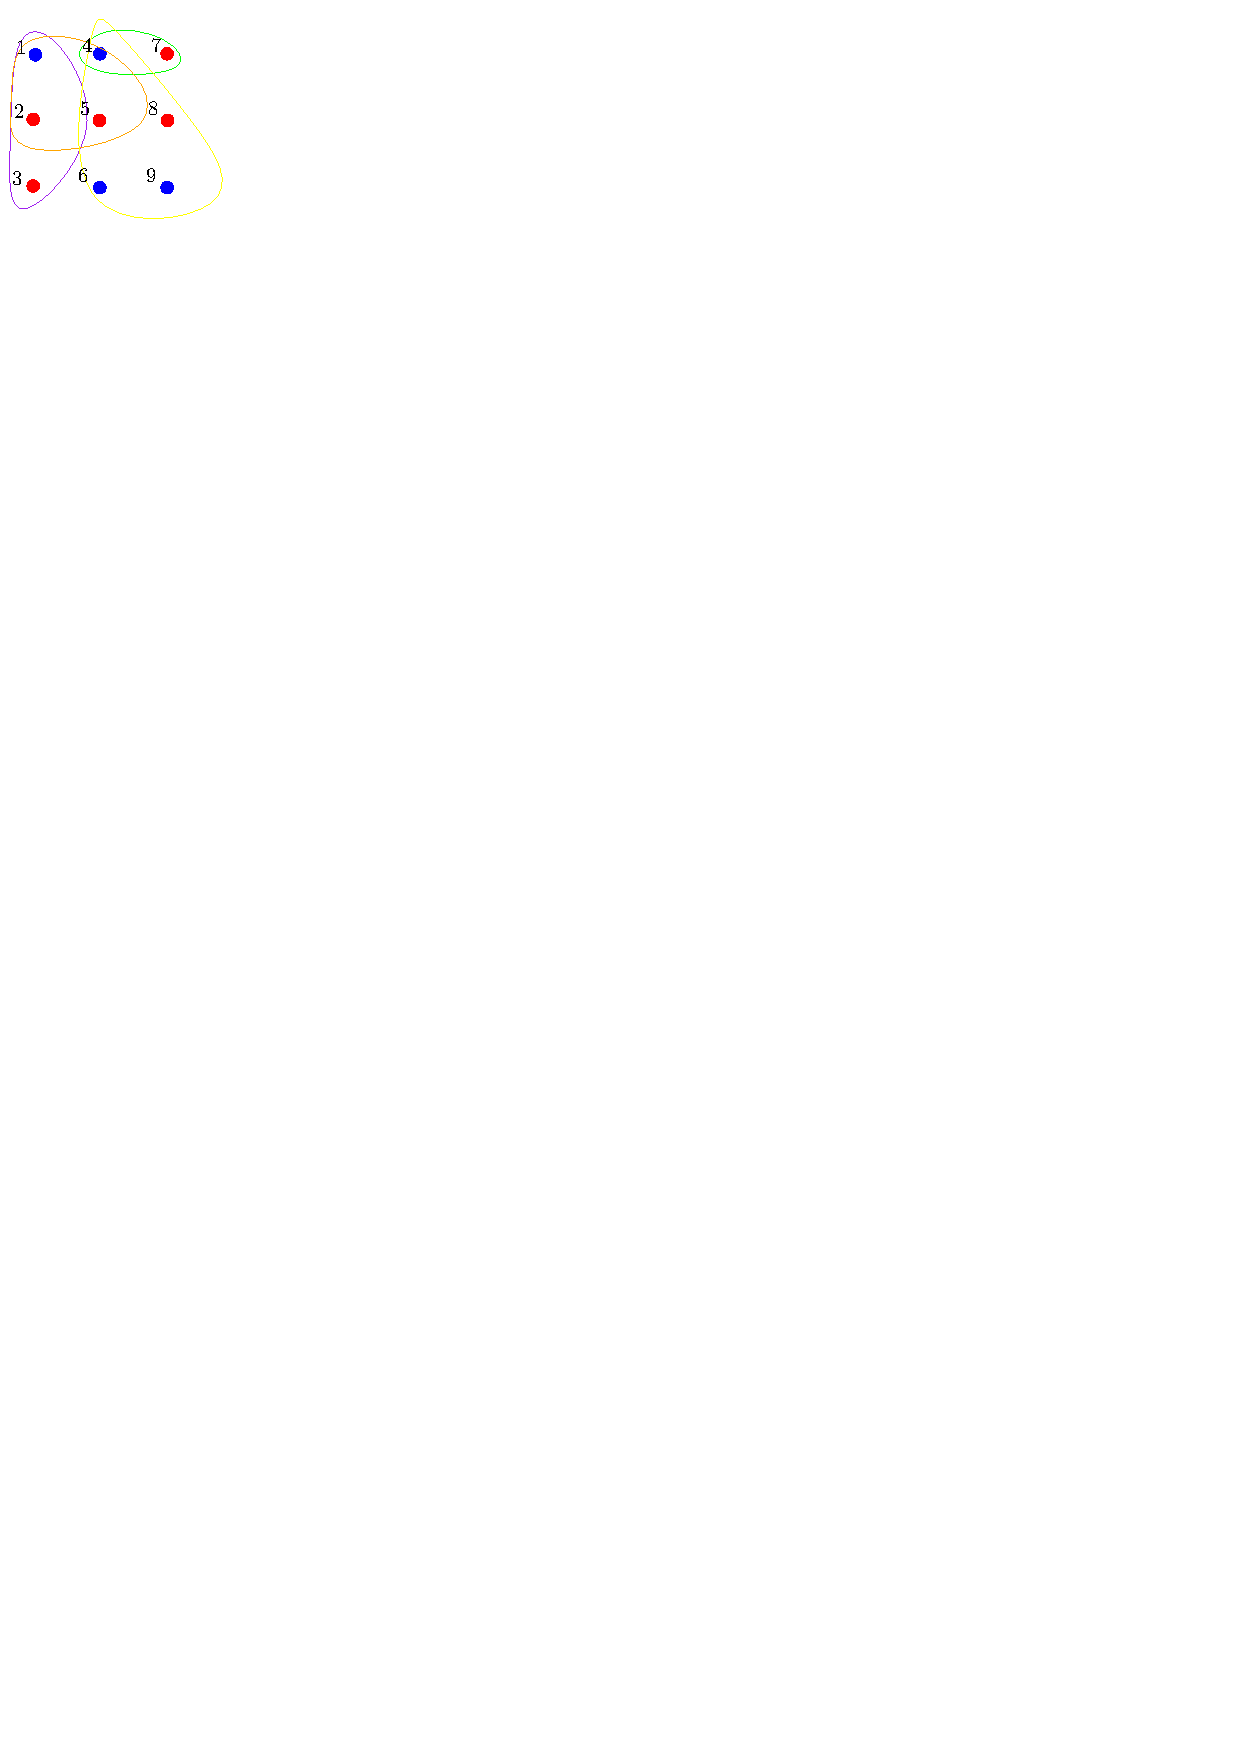
\includegraphics{setsystemnums}    
      \end{center}
  }
  \only<3-4>{
    \begin{align*}
    \left(
      \begin{array}{+c=c=c=c=c=c=c=c=c}
        1 & 2 & 3 & 4 & 5 & 6 & 7 & 8 & 9 \\
        \hline
        \rowstyle{\color{BlueViolet}}
        1 & 1 & 1 & 0 & 0 & 0 & 0 & 0 & 0 \\
        \rowstyle{\color{orange}}
        1 & 1 & 0 & 1 & 1 & 0 & 0 & 0 & 0 \\
        \rowstyle{\color{Lime}}
        0 & 0 & 0 & 1 & 0 & 0 & 1 & 0 & 0 \\
        \rowstyle{\color{yellow}}
        0 & 0 & 0 & 1 & 1 & 1 & 1 & 1 & 1 \\
      \end{array}
    \right) 
    \left(
      \begin{array}{r}
        \color{blue}{-1}\\
        \color{red}{1}\\
        \color{red}{1}\\
        \color{blue}{-1}\\
        \color{red}{1}\\
        \color{blue}{-1}\\
        \color{red}{1}\\
        \color{red}{1}\\
        \color{blue}{-1}\\
      \end{array}
    \right)
    = \left(
      \begin{array}{r}
        \color{red}{1}\\
        0\\
        0\\
        \color{blue}{-1}\\
      \end{array}
    \right)
  \end{align*}
  }
  \only<3>{
    \vspace{4em}
  }
  \only<4>{
    \begin{equation*}
      \disc(\SS) = \disc(U, \|\cdot\|_\infty) = 
      \min_{\eps \in \{\pm 1\}^N}{\|U\eps\|_\infty}
    \end{equation*}
    Natural to consider arbitrary matrices and norms.
  }

}

\junk{\frame{

  \frametitle{Variants}
  
  \textbf{Natural extensions}:
  \begin{itemize}
  \item Discrepancy of an \emph{arbitrary matrix}:\\
    $\disc(U) = \min_{\eps \in \{\pm 1\}^N}{\|U\eps\|_\infty}$. \pause

  \item Discrepancy with respect to an \emph{arbitrary norm} $\|\cdot\|$:
    $\disc(U, \|\cdot\| ) = \min_{\eps \in \{\pm 1\}^N}{\|U\eps\|}$. 
    \begin{itemize}
    \item Studied for $\ell_p$ norms~\mycite{Matousek98-Lp-beckfiala,Larsen17}.
    \end{itemize}\pause
  \end{itemize}
  \medskip

  \textbf{Issues:} Discrepancy is
  \begin{itemize}
  \item not robust to slight changes in the set system
  \item hard to estimate~\mycite{CNN11}
  \end{itemize}\pause
  We need a \emph{robust} version of discrepancy.\pause

  \smallskip
  \textbf{Hereditary Discrepancy} \mycite{LSV}:\\
  $\hd(U, \|\cdot\|) = \max_{S \subseteq [N]} \disc(U_S, \|\cdot\|)$
  \begin{itemize}
  \item $U_S = (u_i)_{i \in S}$.
  \end{itemize}

}}% end junk

\frame{

  \frametitle{Applications}
  
  \begin{itemize}
  \item Constructing uniformly distributed pointsets \mycite{beck-rect}:
    \begin{itemize}
    \item Used in numerical integration (the quasi-Monte Carlo Method);
    \end{itemize}
    \smallskip\pause
    
  \item Constructing {$\epsilon$-nets} \mycite{matousek1995approximations}:
    \begin{itemize}
    \item Used in computational geometry, machine learning;
    \end{itemize}
    \smallskip\pause

  \item Applications in combinatorial optimization: approximation
    algorithms and integrality gaps for
    \begin{itemize}
    \item bin packing~\mycite{HobergRothvoss17,NNN12} and generalizations~\mycite{R12};
    \item {broadcast  scheduling}~\mycite{bcast-scheduling};
    \end{itemize}
    \smallskip\pause
    
  \item Lower bounds for data structures:
    \begin{itemize}
    \item Time to keep dynamic range counts \mycite{disc-larsen};
    \item Space for approximate range counts \mycite{disc-spacelb};
    \end{itemize}
    \smallskip\pause

  \item Algorithms and lower bounds for private data analysis~\mycite{NTZ,smalldb}.
    
  \end{itemize}
}

\frame{

  \frametitle{Basic Bounds}

  \begin{itemize}
  \item \mycite{Spencer, gluskin}: $\disc(\SS) \lesssim  \sqrt{n}$\pause

    \medskip
  \item \emph{Implied by}: For any $u_1, \ldots, u_N \in B_\infty^n = [-1,1]^n$,
    there exist $\eps_1, \ldots, \eps_N \in \{-1, +1\}$ s.t.
    $\|\eps_1 u_1 + \ldots + \eps_N u_N\|_\infty \lesssim
    \sqrt{n}$. \pause

    \bigskip

  \item \mycite{beckfiala}: If every element of $\cal X$ appears in at
    most $t$ sets of $\SS$, then $\disc(\SS) \le 2t - 1$\pause

    \medskip
  \item \emph{Implied by}: For any $u_1, \ldots, u_N \in B_1^n$,
    there exist $\eps_1, \ldots, \eps_N \in \{-1, +1\}$ s.t.
    $\|\eps_1 u_1 + \ldots + \eps_N u_N\|_\infty < 2$. \pause

  \end{itemize}

  \bigskip
  Most combinatorial discrepancy bounds are implied by geometric
  vector balancing arguments. 

}


\frame{

  \frametitle{The Vector Balancing Problem}

  Given $u_1, \ldots, u_N \in \R^n$, and
  symmetric convex body $K\subset \R^n$ ($K = -K$), find the smallest~$t$ such
  that 
  %\vspace{-0.5em}
  \[
  \exists\ \eps_1, \ldots, \eps_N \in \{-1, +1\}: 
  \eps_1 u_1 + \ldots + \eps_N u_N \in tK
  \]

  \begin{center}
    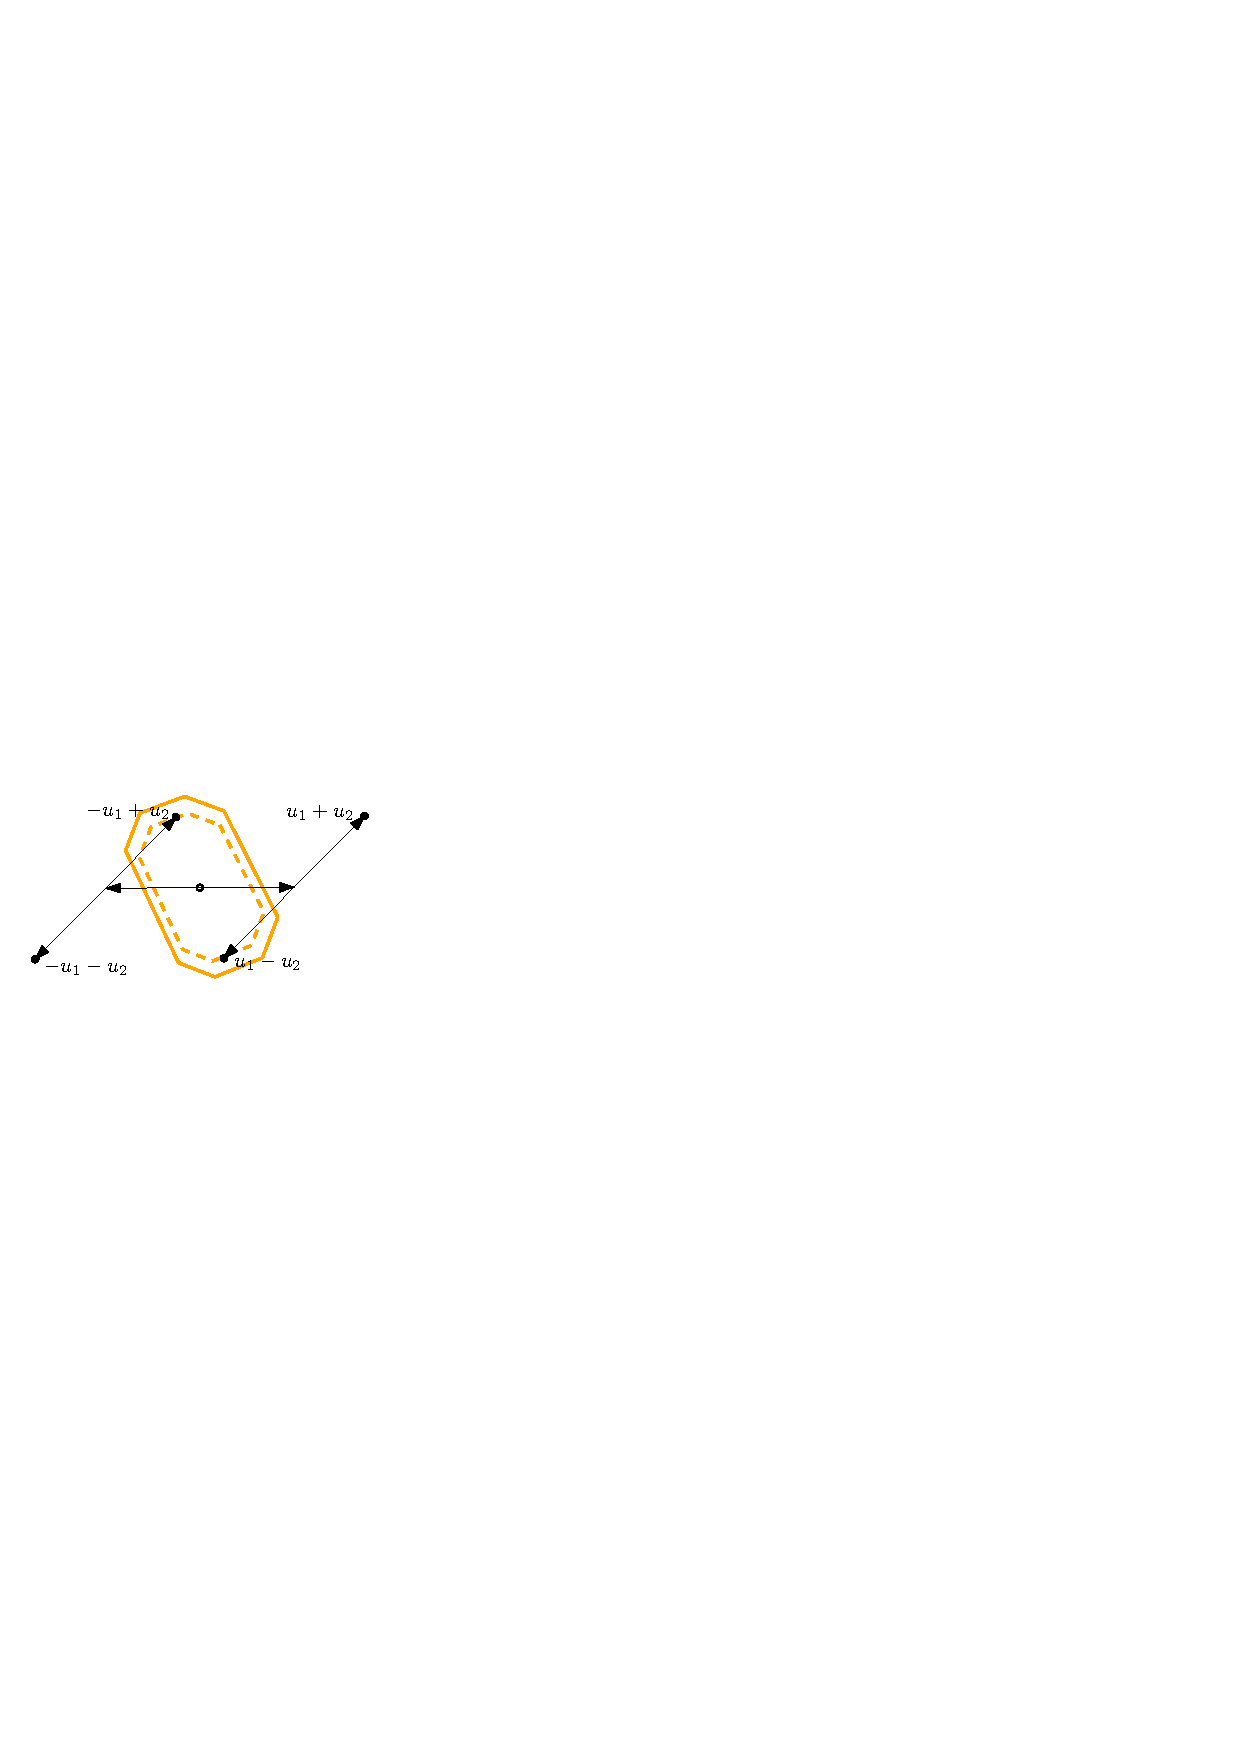
\includegraphics[scale=0.8]{vb}
  \end{center}\pause

  \textbf{Minkowski Norm}: $\|x\|_K = \inf\{t\ge 0: x \in tK\}$;~$t =
  \disc((u_i)_{i = 1}^N, \|\cdot\|_K)$.\pause

  \smallskip
  \textbf{Vector Balancing Constant}: worst case over
  sequences in $C$
  \begin{align*}
  \vb(C, K) &= 
  %\sup\Bigg\{ 
  %\min_{\eps_1, \ldots, \eps_N \in \{-1,1\}} 
  %\Bigl\|\sum_{i = 1}^N \eps_i u_i \Bigr\|_{K}: 
  %N \in \mathbb{N}, u_1, \ldots, u_N \in C \Bigg\}\\
  %&=
  \sup\Bigg\{ 
  \disc(U, \|\cdot\|_K): 
  N \in \mathbb{N}, u_1, \ldots, u_N \in C, U= (u_i)_{i = 1}^N \Bigg\}
  \end{align*}

}

\frame{

  \frametitle{Questions and Prior Results}

  \begin{itemize}
  \item \mycite{Dvoretzky-problem} ``What can be said'' about
    $\vb(K,K)$?
    
    \smallskip
  \item \mycite{baranygrinberg} $\vb(K, K) \le n$ for all $K$.
    \pause

    \medskip
  \item \mycite{Spencer, gluskin} $\vb(B_\infty^n, B_\infty^n)
    \lesssim \sqrt{n}$\

    \smallskip
  \item \mycite{beckfiala} $\vb(B_1^n, B_\infty^n) < 2$
    \pause

    \medskip
  \item \mycite{bana} $vb(B_2^n, K)\le 5$ if $K$ has Gaussian~measure~$\gamma_n(K) \ge \frac12$

    \smallskip
  \item \emph{The Koml\'os Problem}: Prove or disprove $\vb(B_2^n, B_\infty^n) \lesssim 1$.
    \begin{itemize}
    \item Banaszczyk's theorem implies $\vb(B_2^n, B_\infty^n)
      \lesssim \sqrt{\log 2n}$. 
    \end{itemize}
  \end{itemize}

}

\frame{

  \frametitle{Our Results}
  
  We initiate a study of the \emph{computational complexity} of $\vb(C,K)$:\pause
  
  \begin{itemize}
  \item An efficient algorithm to compute 
    $\eps \in \{-1, 1\}^N$ given $u_1, \ldots, u_N \in C$, so that
    $\|\eps_1 u_1 + \ldots + \eps_N u_N\|_K \lesssim (1 + \log n) \vb(C,K)$
    \pause

    \medskip
  \item \alert<6>{An efficient approximation algorithm for $\vb(C,K)$, with
    approximation factor polynomial in $\log n$.}
    \pause

    \medskip
  \item {The results extend to a robust ``hereditary'' version of
    discrepancy with respect to arbitrary norms.}
  \end{itemize}\pause

  {Prior work~\mycite{Bansal10,NT15} implies bounds which deteriorate
  with the number of facets of $K$, rather than dimension. 

  \medskip
  Our work exploits the geometry of the problem more fully. }\pause
}


\section{Upper Bound}

\frame{
  
  \frametitle{How to Bound $\vb(C,K)$ from above?}

  $\vb(C,K)$ is a maximum over all sequences $(u_i)_{i, N}$ of points
  from $C$.

  \smallskip
  \emph{How can we prove an upper bound on $\vb(C,K)$?}\pause
  
  \bigskip
  Recall \mycite{bana}:\\ For any convex $K \subset \R^n$ such that
  $\gamma_n(K) \ge \frac12$, $\vb(B_2^n, K) \le 5$.\pause

  \bigskip
  \textbf{Observations}:
  \begin{itemize}
  \item If $\E \|G\|_K\le 1$ for $G \sim N(0,I_n)$, then
    \vspace{-1em}
    \[
    \gamma_n(2K) = \Pr(\|G\|_K \le 2) \ge \frac12.
    \]

    \vspace{-1em}
  \item $\vb(B_2^n, K) \lesssim \E \|G\|_K$.
    %\pause
    %\smallskip
    
  %\item $\vb(C, K) \lesssim (\E \|G\|_K) \cdot
  %  \mathrm{diam}_{\ell_2}(C)$.
  \end{itemize}
  %Last 

}

\frame{

  \frametitle{Upper Bound for Abritrary $C$}

  \begin{itemize}
  \item Say $C \subseteq R\cdot B_2^n$: 
    %\vspace{-1em}
    $
    \vb(C, K) \leq \vb(R\cdot B_2, K) = R \cdot\vb(B_2, K).
    $%\pause

    %\vspace{-1em}
      \begin{center}
        \includegraphics{UB-ball}
      \end{center}\pause
    

  \item $\vb(C, K) \lesssim (\E \|G\|_K) \cdot
    \mathrm{diam}_{\ell_2}(C)$.\pause

  \item 
    \begin{minipage}{0.6\linewidth}
        This bound can be very loose!
      \end{minipage}
      \begin{minipage}{0.3\linewidth}
        \includegraphics{UB-ball-bad}
      \end{minipage}
      


  \end{itemize}

}

\frame{
  
  \frametitle{A Better Upper Bound}
  \begin{minipage}{0.5\linewidth}
  \textbf{Idea}: Fit an \emph{ellipsoid} around $C$.    
  \end{minipage}\pause
  \begin{minipage}{0.4\linewidth}
  \begin{center}
    \includegraphics[scale=0.8]{UB-ellipsoid}
  \end{center}\pause
  \end{minipage}

  

  \begin{itemize}
  \item Let $C \subseteq E = AB_2^n$ for a linear map $A$:
    \[
    \vb(C, K) \le \vb(E, K) = \vb(A^{-1}E, A^{-1}K) 
    = \vb(B_2^n, A^{-1}K).
    \]

  \item We can apply Banaszczyk's Theorem: $\vb(C, K) \lesssim
    \E\|G\|_{A^{-1}K}$. \pause

  \item \textbf{General upper bound:}
    \vspace{-0.8em}
    \[
    \lambda(C,K) = 
    \inf\{ \E \|G\|_{F(K)}:
    F \text{ a linear map}, F(C) \subseteq B_2^n\}.
    \]
  \end{itemize}
  

  
  \junk{
  \textbf{Claim}: $\vb(C,K) \lesssim \lambda(C,K)$.\pause

  \smallskip
  \begin{itemize}
  \item Take a linear map $F$ achieving $\lambda(C, K)$;
    \begin{itemize}
    \item Can assume $\mathrm{diam}_{\ell_2}(F(C)) = 1$, 
      so $\E \|G\|_{F(K)} = \lambda(C,K)$;
    \end{itemize}\pause
  \item $\vb(C,K) = \vb(F(C), F(K))$ and apply Banaszczyk's theorem.
  \end{itemize}
  }
}

%\section{Dual and Tightness}

\frame{
  \frametitle{Tightness of the Upper Bound}

  \begin{theorem}
    For any symmetric convex $C, K \subset \R^n$,
    \vspace{-1em}
    \begin{align*}
      \frac{\lambda(C,K) }{(1+\log n)^{5/2}} 
      \lesssim \vb(C, K) 
      \lesssim \lambda(C,K).
    \end{align*}
    Moreover, given membership oracle access to $K$ and a vertex
    representation of $C$, we can efficiently compute $\lambda(C,K)$. 
  \end{theorem}
  \pause

  \smallskip
  \textbf{Proof outline}:
  \begin{enumerate}
  \item Formulate $\lambda(C,K)$ as a convex minimization problem;
  \item Derive the Lagrange dual: an equivalent maximization problem;
    %\begin{itemize}
    %\item Dual solutions give lower bounds on $\lambda(C,K)$;
    %\end{itemize}
  \item Relate dual solutions to lower bounds on $\vb(C,K)$.
  \end{enumerate}
}

\frame{
  \frametitle{Convex Formulation}

  $\|x\|_{F(K)} = \|F^{-1}x\|_K$

  \smallskip
  \textbf{First attempt}: $\inf\{\E \|F^{-1}G\|_K: F(C) \subseteq B_2^n \}$
  \begin{itemize}
  \item \emph{Not convex}: the objective is $\infty$ for $F = 0$,
    finite for any invertible $F$, but $0 = \frac12(F + (-F))$. 
  \end{itemize}\pause

  \smallskip
  \textbf{Observation}: $\E \|F^{-1}G\|_K$ is defined
  entirely by $M = F^\intercal F$, because the covariance of
  $F^{-1}G$ is $M^{-1}$. \pause

  \smallskip
  \textbf{Formulation}:
  \vspace{-2em}
  \begin{align*}
    \lambda(C,K) = &\inf  f(M) \\
    \text{s.t.\ \ }
    &u^\intercal M u \le 1 \ \ \ \forall u \in C\\
    &A \succ 0.
  \end{align*}
  
  \vspace{-1em}
  \begin{itemize}
  \item $f(M) = \E \|F^{-1}G\|_K$ for any $F$ such that
    $F^\intercal F = M$;
    \begin{itemize}
    \item $f$ is well defined and convex;
    \end{itemize}\pause

  \item The first constraint encodes $ F(C) \subseteq B_2^n$: 
    $u^\intercal M u =  u^\intercal F^\intercal F u  = \|Fu\|_2^2$.
  \end{itemize}

}

\frame{

  \frametitle{Computation}

\begin{align*}
    \lambda(C,K) = &\inf  f(M) \\
    \text{s.t.\ \ }
    &u^\intercal M u \le 1 \ \ \ \forall u \in C\\
    &A \succ 0.
  \end{align*}
  
  Solved by the Ellipsoid method:\pause
  \begin{itemize}
  \item We first put $C$ in John's position 
    ($B_2^n \subseteq C \subseteq \sqrt{n}B_2^n$), 
    so that the problem is well-conditioned.\pause

  \item We can approximate $f(M) = \E \|F^{-1} G\|_K$ by sampling.\pause

  \item Given a vertex representation for $C$, we can check 
    $u^\intercal M u \le 1 \ \ \ \forall u \in C$ efficiently.

  \end{itemize}

}

\frame{
  
  \frametitle{Dual Formulation}
  
  \begin{itemize}
  %\item The function $f(A)$ is convex in $A$, and the constraints are  also convex;

  \item \textbf{Lagrange Duality}: there exists an
    \emph{equivalent} dual problem
    \begin{align*}
      \lambda(C, K) &= \sup \tr((R(\sum_{i = 1}^m{p_i u_i u_i^\intercal })R^\intercal)^{1/3})^{3/2}\\
      \text{s.t.}\ \ \ 
      &u_1, \ldots, u_m \in C\\
      &\tr(RT)\le 1 \ \ \ \forall T 
      \text{ s.t. }  \E \|TG\|_K \le 1\\
      &\sum_{i = 1}^m{p_i} = 1, \ \ 
      p_1, \ldots, p_m \ge 0. 
    \end{align*}\pause



    %dual maximization problem, whose value also equals
    %$\lambda(U,C)$;\pause

    \vspace{-0.8em}
  \item From each dual solution we extract a volumetric lower bound on $\vb(C,K)$;
    \begin{itemize}
    \item Tools: $K$-convexity, and Sudakov minoration;
    \end{itemize}

  \item $\implies$ $\lambda(C,K)$ gives a lower bound on $\vb(C,K)$
    (up to $\log n$ factors).
  \end{itemize}

  %\textbf{Computation}: The convex optimization problem can be solved
  %using the ellipsoid method, given a membership oracle for $K$ and a
  %vertex representation of $C$.
  
}

\section{Conclusion}

\frame{

  \frametitle{Conclusion}

  \textbf{In this work}:
  \begin{itemize}
  \item Efficient algorithms to find nearly optimal vector balancing
    signs, and to compute $\vb(C,K)$. 

  \item Our results strongly use the geometry of the underlying
    discrepancy problem. 
  \end{itemize}\pause

  \textbf{Open questions}:
  \begin{itemize}
  \item Hardness of approximation?
  \item Can the bounds for $\lambda(C,K)$ be improved?
  \end{itemize}
}

\bibliographystyle{plainnat}
\bibliography{../Discrepancy}

\end{document}


